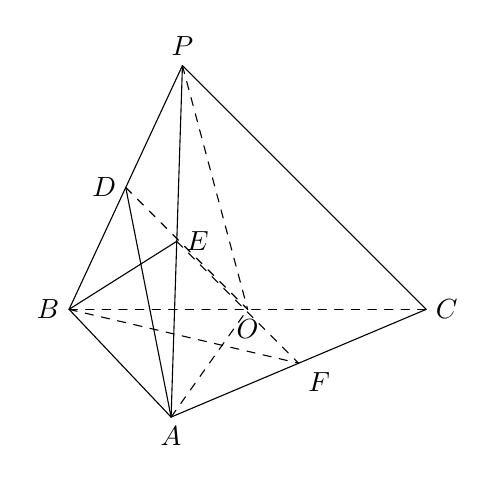
\begin{tikzpicture}[x=0.72cm,y=0.72cm,line cap=round,line join=round]
  \coordinate (P) at (2.0,6.6);
  \coordinate (A) at (1.8,0.4);
  \coordinate (B) at (0,2.3);
  \coordinate (C) at (6.3,2.3);
  \coordinate (D) at (1.0,4.45);
  \coordinate (E) at (1.9,3.5);
  \coordinate (O) at (3.15,2.3);
  \coordinate (F) at (4.05,1.35);

  % 三棱锥外棱及面内可见线
  \draw (P)--(B)--(A)--(C)--(P);
  \draw (P)--(A);
  \draw (D)--(A);
  \draw (B)--(E);
  \draw[dashed] (E)--(F);

  % 原图中的遮挡线
  \draw[dashed] (B)--(C);
  \draw[dashed] (P)--(O);
  \draw[dashed] (D)--(O);
  \draw[dashed] (A)--(O);
  \draw[dashed] (B)--(F);

  \node[above] at (P) {$P$};
  \node[below] at (A) {$A$};
  \node[left] at (B) {$B$};
  \node[right] at (C) {$C$};
  \node[left] at (D) {$D$};
  \node[right] at (E) {$E$};
  \node[below] at (O) {$O$};
  \node[below right] at (F) {$F$};
\end{tikzpicture}
